%
% main.tex -- Paper zum Thema <rossby>
%
% (c) 2020 Autor, OST Ostschweizer Fachhochschule
%
% !TEX root = ../../buch.tex
% !TEX encoding = UTF-8
%
\chapter{Rossby Wellen\label{chapter:rossby}}
\kopflinks{Rossby Wellen}
\begin{refsection}
\chapterauthor{Michael Schmid}

\subparagraph{Die Vortizitätsgleichung}
\begin{equation}
  \zeta = \frac{\partial v}{\partial x} - \frac{\partial u}{\partial y}
\end{equation}

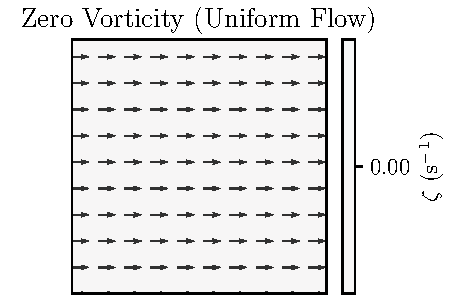
\includegraphics[]{papers/rossby/images/vorticity_plot0.pdf}

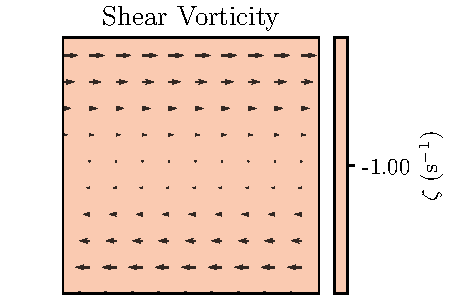
\includegraphics[]{papers/rossby/images/vorticity_plot1.pdf}

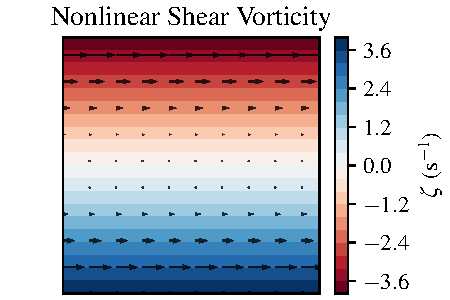
\includegraphics[]{papers/rossby/images/vorticity_plot2.pdf}

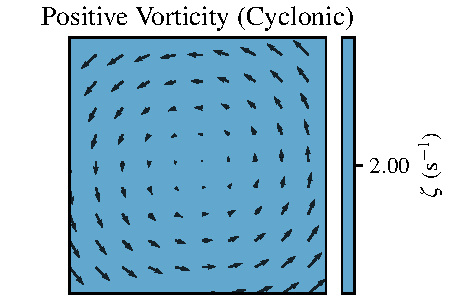
\includegraphics[]{papers/rossby/images/vorticity_plot3.pdf}

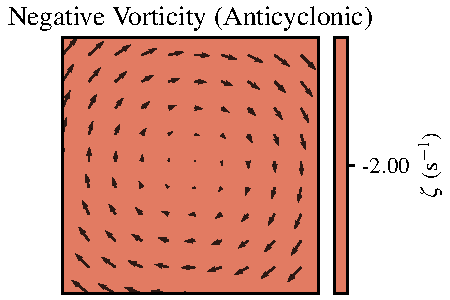
\includegraphics[]{papers/rossby/images/vorticity_plot4.pdf}

\printbibliography[heading=subbibliography]
\end{refsection}
